\documentclass[a4paper]{article}

\def\npart{II}

\def\ntitle{Graph Theory}
\def\nlecturer{P.\ A.\ Russel}

\def\nterm{Michaelmas}
\def\nyear{2018}

\ifx \nauthor\undefined
  \def\nauthor{Qiangru Kuang}
\else
\fi

\ifx \ntitle\undefined
  \def\ntitle{Template}
\else
\fi

\ifx \nauthoremail\undefined
  \def\nauthoremail{qk206@cam.ac.uk}
\else
\fi

\ifx \ndate\undefined
  \def\ndate{\today}
\else
\fi

\title{\ntitle}
\author{\nauthor}
\date{\ndate}

%\usepackage{microtype}
\usepackage{mathtools}
\usepackage{amsthm}
\usepackage{stmaryrd}%symbols used so far: \mapsfrom
\usepackage{empheq}
\usepackage{amssymb}
\let\mathbbalt\mathbb
\let\pitchforkold\pitchfork
\usepackage{unicode-math}
\let\mathbb\mathbbalt%reset to original \mathbb
\let\pitchfork\pitchforkold

\usepackage{imakeidx}
\makeindex[intoc]

%to address the problem that Latin modern doesn't have unicode support for setminus
%https://tex.stackexchange.com/a/55205/26707
\AtBeginDocument{\renewcommand*{\setminus}{\mathbin{\backslash}}}
\AtBeginDocument{\renewcommand*{\models}{\vDash}}%for \vDash is same size as \vdash but orginal \models is larger
\AtBeginDocument{\let\Re\relax}
\AtBeginDocument{\let\Im\relax}
\AtBeginDocument{\DeclareMathOperator{\Re}{Re}}
\AtBeginDocument{\DeclareMathOperator{\Im}{Im}}
\AtBeginDocument{\let\div\relax}
\AtBeginDocument{\DeclareMathOperator{\div}{div}}

\usepackage{tikz}
\usetikzlibrary{automata,positioning}
\usepackage{pgfplots}
%some preset styles
\pgfplotsset{compat=1.15}
\pgfplotsset{centre/.append style={axis x line=middle, axis y line=middle, xlabel={$x$}, ylabel={$y$}, axis equal}}
\usepackage{tikz-cd}
\usepackage{graphicx}
\usepackage{newunicodechar}

\usepackage{fancyhdr}

\fancypagestyle{mypagestyle}{
    \fancyhf{}
    \lhead{\emph{\nouppercase{\leftmark}}}
    \rhead{}
    \cfoot{\thepage}
}
\pagestyle{mypagestyle}

\usepackage{titlesec}
\newcommand{\sectionbreak}{\clearpage} % clear page after each section
\usepackage[perpage]{footmisc}
\usepackage{blindtext}

%\reallywidehat
%https://tex.stackexchange.com/a/101136/26707
\usepackage{scalerel,stackengine}
\stackMath
\newcommand\reallywidehat[1]{%
\savestack{\tmpbox}{\stretchto{%
  \scaleto{%
    \scalerel*[\widthof{\ensuremath{#1}}]{\kern-.6pt\bigwedge\kern-.6pt}%
    {\rule[-\textheight/2]{1ex}{\textheight}}%WIDTH-LIMITED BIG WEDGE
  }{\textheight}% 
}{0.5ex}}%
\stackon[1pt]{#1}{\tmpbox}%
}

%\usepackage{braket}
\usepackage{thmtools}%restate theorem
\usepackage{hyperref}

% https://en.wikibooks.org/wiki/LaTeX/Hyperlinks
\hypersetup{
    %bookmarks=true,
    unicode=true,
    pdftitle={\ntitle},
    pdfauthor={\nauthor},
    pdfsubject={Mathematics},
    pdfcreator={\nauthor},
    pdfproducer={\nauthor},
    pdfkeywords={math maths \ntitle},
    colorlinks=true,
    linkcolor={red!50!black},
    citecolor={blue!50!black},
    urlcolor={blue!80!black}
}

\usepackage{cleveref}



% TODO: mdframed often gives bad breaks that cause empty lines. Would like to switch to tcolorbox.
% The current workaround is to set innerbottommargin=0pt.

%\usepackage[theorems]{tcolorbox}





\usepackage[framemethod=tikz]{mdframed}
\mdfdefinestyle{leftbar}{
  %nobreak=true, %dirty hack
  linewidth=1.5pt,
  linecolor=gray,
  hidealllines=true,
  leftline=true,
  leftmargin=0pt,
  innerleftmargin=5pt,
  innerrightmargin=10pt,
  innertopmargin=-5pt,
  % innerbottommargin=5pt, % original
  innerbottommargin=0pt, % temporary hack 
}
%\newmdtheoremenv[style=leftbar]{theorem}{Theorem}[section]
%\newmdtheoremenv[style=leftbar]{proposition}[theorem]{proposition}
%\newmdtheoremenv[style=leftbar]{lemma}[theorem]{Lemma}
%\newmdtheoremenv[style=leftbar]{corollary}[theorem]{corollary}

\newtheorem{theorem}{Theorem}[section]
\newtheorem{proposition}[theorem]{Proposition}
\newtheorem{lemma}[theorem]{Lemma}
\newtheorem{corollary}[theorem]{Corollary}
\newtheorem{axiom}[theorem]{Axiom}
\newtheorem*{axiom*}{Axiom}

\surroundwithmdframed[style=leftbar]{theorem}
\surroundwithmdframed[style=leftbar]{proposition}
\surroundwithmdframed[style=leftbar]{lemma}
\surroundwithmdframed[style=leftbar]{corollary}
\surroundwithmdframed[style=leftbar]{axiom}
\surroundwithmdframed[style=leftbar]{axiom*}

\theoremstyle{definition}

\newtheorem*{definition}{Definition}
\surroundwithmdframed[style=leftbar]{definition}

\newtheorem*{slogan}{Slogan}
\newtheorem*{eg}{Example}
\newtheorem*{ex}{Exercise}
\newtheorem*{remark}{Remark}
\newtheorem*{notation}{Notation}
\newtheorem*{convention}{Convention}
\newtheorem*{assumption}{Assumption}
\newtheorem*{question}{Question}
\newtheorem*{answer}{Answer}
\newtheorem*{note}{Note}
\newtheorem*{application}{Application}

%operator macros

%basic
\DeclareMathOperator{\lcm}{lcm}

%matrix
\DeclareMathOperator{\tr}{tr}
\DeclareMathOperator{\Tr}{Tr}
\DeclareMathOperator{\adj}{adj}

%algebra
\DeclareMathOperator{\Hom}{Hom}
\DeclareMathOperator{\End}{End}
\DeclareMathOperator{\id}{id}
\DeclareMathOperator{\im}{im}
\DeclarePairedDelimiter{\generation}{\langle}{\rangle}

%groups
\DeclareMathOperator{\sym}{Sym}
\DeclareMathOperator{\sgn}{sgn}
\DeclareMathOperator{\inn}{Inn}
\DeclareMathOperator{\aut}{Aut}
\DeclareMathOperator{\GL}{GL}
\DeclareMathOperator{\SL}{SL}
\DeclareMathOperator{\PGL}{PGL}
\DeclareMathOperator{\PSL}{PSL}
\DeclareMathOperator{\SU}{SU}
\DeclareMathOperator{\UU}{U}
\DeclareMathOperator{\SO}{SO}
\DeclareMathOperator{\OO}{O}
\DeclareMathOperator{\PSU}{PSU}

%hyperbolic
\DeclareMathOperator{\sech}{sech}

%field, galois heory
\DeclareMathOperator{\ch}{ch}
\DeclareMathOperator{\gal}{Gal}
\DeclareMathOperator{\emb}{Emb}



%ceiling and floor
%https://tex.stackexchange.com/a/118217/26707
\DeclarePairedDelimiter\ceil{\lceil}{\rceil}
\DeclarePairedDelimiter\floor{\lfloor}{\rfloor}


\DeclarePairedDelimiter{\innerproduct}{\langle}{\rangle}

%\DeclarePairedDelimiterX{\norm}[1]{\lVert}{\rVert}{#1}
\DeclarePairedDelimiter{\norm}{\lVert}{\rVert}



%Dirac notation
%TODO: rewrite for variable number of arguments
\DeclarePairedDelimiterX{\braket}[2]{\langle}{\rangle}{#1 \delimsize\vert #2}
\DeclarePairedDelimiterX{\braketthree}[3]{\langle}{\rangle}{#1 \delimsize\vert #2 \delimsize\vert #3}

\DeclarePairedDelimiter{\bra}{\langle}{\rvert}
\DeclarePairedDelimiter{\ket}{\lvert}{\rangle}




%macros

%general

%divide, not divide
\newcommand*{\divides}{\mid}
\newcommand*{\ndivides}{\nmid}
%vector, i.e. mathbf
%https://tex.stackexchange.com/a/45746/26707
\newcommand*{\V}[1]{{\ensuremath{\symbf{#1}}}}
%closure
\newcommand*{\cl}[1]{\overline{#1}}
%conjugate
\newcommand*{\conj}[1]{\overline{#1}}
%set complement
\newcommand*{\stcomp}[1]{\overline{#1}}
\newcommand*{\compose}{\circ}
\newcommand*{\nto}{\nrightarrow}
\newcommand*{\p}{\partial}
%embed
\newcommand*{\embed}{\hookrightarrow}
%surjection
\newcommand*{\surj}{\twoheadrightarrow}
%power set
\newcommand*{\powerset}{\mathcal{P}}

%matrix
\newcommand*{\matrixring}{\mathcal{M}}

%groups
\newcommand*{\normal}{\trianglelefteq}
%rings
\newcommand*{\ideal}{\trianglelefteq}

%fields
\renewcommand*{\C}{{\mathbb{C}}}
\newcommand*{\R}{{\mathbb{R}}}
\newcommand*{\Q}{{\mathbb{Q}}}
\newcommand*{\Z}{{\mathbb{Z}}}
\newcommand*{\N}{{\mathbb{N}}}
\newcommand*{\F}{{\mathbb{F}}}
%not really but I think this belongs here
\newcommand*{\A}{{\mathbb{A}}}

%asymptotic
\newcommand*{\bigO}{O}
\newcommand*{\smallo}{o}

%probability
\newcommand*{\prob}{\mathbb{P}}
\newcommand*{\E}{\mathbb{E}}

%vector calculus
\newcommand*{\gradient}{\V \nabla}
\newcommand*{\divergence}{\gradient \cdot}
\newcommand*{\curl}{\gradient \cdot}

%logic
\newcommand*{\yields}{\vdash}
\newcommand*{\nyields}{\nvdash}

%differential geometry
\renewcommand*{\H}{\mathbb{H}}
\newcommand*{\transversal}{\pitchfork}
\renewcommand{\d}{\mathrm{d}} % exterior derivative

%number theory
\newcommand*{\legendre}[2]{\genfrac{(}{)}{}{}{#1}{#2}}%Legendre symbol


\newcommand*{\Omg}{\Omega}
\newcommand*{\bigT}{\Theta}
\newcommand*{\smallomg}{\omega}
\DeclareMathOperator{\exx}{ex} % forbidden subgraph notation

\let\SO\undefined
\usepackage{tkz-graph}

\begin{document}

\begin{titlepage}
  \begin{center}
    
\includegraphics[width=0.6\textwidth]{logo.jpg}\par
    \vspace{1cm}
    {\scshape\huge Mathematics Tripos \par}
    \vspace{2cm}
    {\huge Part \npart \par}
    \vspace{0.6cm}
    {\Huge \bfseries \ntitle \par}
    \vspace{1.2cm}
    {\Large\nterm, \nyear \par}
    \vspace{2cm}
    
    {\large \emph{Lectures by } \par}
    \vspace{0.2cm}
    {\Large \scshape \nlecturer}
    
    \vspace{0.5cm}
    {\large \emph{Notes by }\par}
    \vspace{0.2cm}
    {\Large \scshape \href{mailto:\nauthoremail}{\nauthor}}
 \end{center}
\end{titlepage}

\tableofcontents

\setcounter{section}{-1}

\section{Introduction}

Informally, a \emph{graph} consists of some vertices with some pairs of ``vertices'' joined by ``edges''. (formal definition later)

A few problems:
\begin{enumerate}
\item bridges of Königsberg (Euler, 18th century): is it possible to walk round the city crossing each bridge precisely once and returing to starting point? Convert it into a graph, the question becomes: is it possible to walk round the ``graph'', traversing each edge precisely once, finishing at the starting vertex?\footnote{This is actually a multigraph, with more than one edge joining two vertices.}
\item four colour problem (first proposed in 19th century): how many colours are needed to colour a map? Denote each country by a vertex and connect two vertices by an edge if the countries are neighbours. Conjecture: let \(G\) be a graph that can be drawn in the plane with no crossings. Then the vertices of \(G\) can be coloured with \(4\) colours such that each edge has different coloured endpoints.
\item simultaneous coset representation (1930s): let \(G\) be a finite group, \(H \leq G\). Lagrange's Theorem says that \(|H| \divides |G|\) and if \(|G|/|H| = n\) then there are \(a_1, \dots, a_n \in G\) such that \(a_1H, \dots, a_nH\) are the left cosets of \(H\). Similarly there exist \(b_1, \dots, b_n \in G\) such that \(Hb_1, \dots, Hb_n\) are the right cosets. We can ask the problem: can we make the \(a_i\)'s and \(b_i\)'s the same? i.e.\ can we find \(c_1, \dots, c_n \in G\) such that the left cosets of \(H\) are \(c_1H, \dots, c_nH\) and the rights cosets are \(Hc_1, \dots, Hc_n\)? Recall that if \(L\) is a left coset of \(H\) and \(g \in G\) then \(L = gH\) if and only if \(g \in L\). Take set \(X\) of vertices, one for each left coset, disjoint set \(Y\) of vertices, one for each right coset. For each \(g \in G\), add an edge from \(gH\) to \(Hg\). The problem now becomes: can we find a set of edges meeting each vertex precisely once?
\item Fermat equation mod \(p\): Fermat asserted that \(x^n + y^n = z^n\) has no non-trivial solutions in integers if \(n \geq 3\). 

  \begin{theorem}
    Let \(n \in \N\). Then for any sufficiently large prime \(p\), there are \(x, y, z \neq 0 \pmod p\) with \(x^n + y^n = z^n \pmod p\).
  \end{theorem}

  The original proof involves lots of number theory and is hard. However we can reduce it to a graph theory problem. Let \(G = \Z_p^*\), multiplicative group of nonzero residues mod \(p\). Let \(H = \{g^n: g \in G\} \leq G\). We want \(x, y, z \in H\) with \(x + y = z\). We can check \(|H| \geq \frac{|G|}{n}\) so \(H\) has at most \(n\) left cosets. Suppose now in some left coset \(gH\) we have \(u, v, w \in gH\) with \(u + v = w\). Then \(g^{-1}u + g^{-1}v = g^{-1}w\) is a solution in \(H\). Thus we have reduced the theorem to the following combinatorial statement:

  \begin{theorem}[Schur]
    Let \(k\) be a positive integer. Then for any sufficiently large \(n\), if \([n] = \{1, 2, \dots, n\}\) is partitioned into \(k\) parts, then we can find \(x, y, z\) in the same part with \(x + y = z\).
  \end{theorem}
\end{enumerate}

Let's consider small cases to gain some intuition first. For \(k = 1\), take \(n = 2\). It is trivial.

For \(k = 2\), take \(n = 5\). Suppose \([5]\) is partitioned into \(A\) and \(B\). wlog \(|A| \geq 3\), say \(i < j < k\) in \(A\). If \(j - i \in A\) then \(i + (j - i) = j\) so done. Similarly if \(k - i \text{ or } k - j \in A\). Otherwise, \(j - i, k - j, k - i \in B\) and \((j - i) + (k - j) = k - i\) so done.

For \(k = 3\), take \(n = 16\). Suppose \([16]\) is partitioned in \(A, B\) and \(C\). wlog \(|A| \geq 6\) and \(a_1 < \dots < a_6\) in \(A\). If \(a_j - a_i \in A\) for some \(i < j\) then done. If not, consider \(a_2 - a_1, a_3 - a_1, \dots, a_6 - a_1 \in B \cup C\) so wlog have \(2 \leq i < j < k < 6\) such that \(a_i - a_1, a_j - a_1, a_k - a_1 \in B\). Now if \(a_j - a_i \text{ or } a_k - a_j \text{ or } a_k - a_i \in B\) then done. Otherwise \(a_j - a_i, a_k - a_j, a_k - a_i \in C\) and so done.

The ``if not'' part of \(k = 3\) feels quite like \(k = 2\) case, except that we are dealing with \(a_i - a_1\) instead of \(1, \dots, 5\). It is a bit tricky but we can do this by induction. This is left as an exercise.

Note that what we care is the difference between the numbers. More specifically, we only care the difference between \emph{a pair} of numbers, instead of what the actual difference is. This prompts us to rephrase this as a graph theory problem. Let \([5] = A \cup B\), say \(A = \{1, 3, 5\}, B = \{2, 4\}\). Take the graph with vertices \(0, \dots, 5\) and all possible edges. Colour the edge \(ij (i < j)\) to represent which of \(A, B\) contains \(j - i\).

\begin{center}
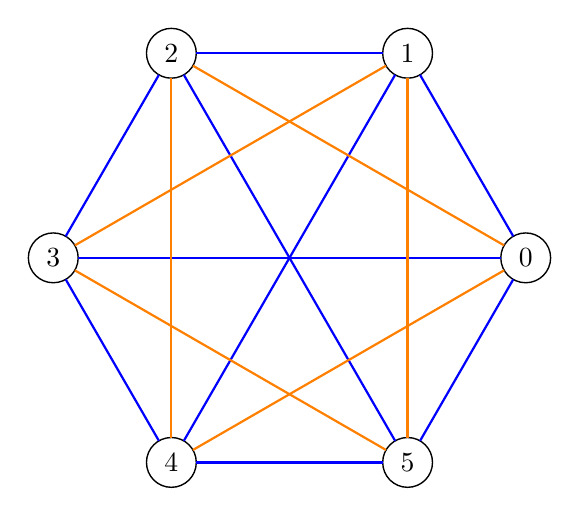
\begin{tikzpicture}
  \SetGraphUnit{3}
  \SetUpEdge[color = blue]
  \Vertices{circle}{0, 1, 2, 3, 4, 5}
  \Edges(0, 1, 2, 3, 4, 5, 0)
  \Edges(0, 3)
  \Edges(1, 4)
  \Edges(2, 5)
  \SetUpEdge[color = orange]
  \Edges(0, 2, 4, 0)
  \Edges(1, 3, 5, 1)
\end{tikzpicture}
\end{center}

Supoose we have a monochromatic triangle \(i < j < k\), then \(j - i, k - j, k - i\) are in the same part with \((k - j) + (j - i) = k - i\). This turns out to be exactly the setting we need to solve this problem. We will do this in chapter 1, alongside building the machinary we need.

\section{Extremal graph theory}

\subsection{Ramsey theory}

\begin{definition}[graph, vertex, edge]\index{graph}
  A \emph{graph} \(G\) is an ordered pair \(G = (V, E)\) where \(V\) is a finite set and \(E\) is a set of unordered pairs of distinct elements of \(V\). The elements of \(V\) are the \emph{vertices} of \(G\) and those of \(E\) the \emph{edges}. Write \(V = V(E)\) and \(E = E(G)\).
\end{definition}

\begin{eg}
  \(G = ([9], \{12, 13, 14, 23, 67, 68, 69\})\). We often use picture to represent a graph.
  \begin{center}
    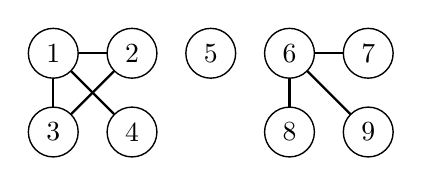
\begin{tikzpicture}
      \SetGraphUnit[3]
      \Vertex{1}
      \Vertex[x=1,y=0]{2}
      \Vertex[x=0,y=-1]{3}
      \Vertex[x=1,y=-1]{4}
      \Edges(1, 2, 3, 1)
      \Edges(1, 4)

      \Vertex[x=2,y=0]{5}

      \Vertex[x=3,y=0]{6}
      \Vertex[x=4,y=0]{7}
      \Vertex[x=3,y=-1]{8}
      \Vertex[x=4,y=-1]{9}
      \Edges(8,6,7)
      \Edges(6,9)
    \end{tikzpicture}
  \end{center}
\end{eg}

\begin{notation}
  We denote the edge \(\{i, j\}\) by \(ij\).
\end{notation}

\begin{eg}
  The \emph{complete graph of order \(n\)} \(K_n\) has \(V[K_n] = [n]\) and \(E(K_n) = \{ij: 1 \leq i < j \leq n\}\). For example, \(K_3\) is the \emph{triangle}\index{triangle}.
  \begin{center}
    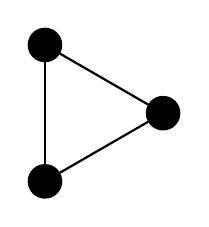
\begin{tikzpicture}
      \GraphInit[vstyle=Classic]
      \Vertices[NoLabel]{circle}{1, 2, 3}
      \Edges(1, 2, 3, 1)
    \end{tikzpicture}

    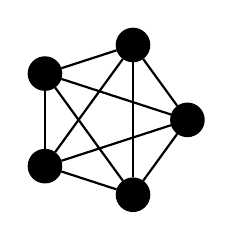
\begin{tikzpicture}
      \GraphInit[vstyle=Classic]
      \Vertices[NoLabel]{circle}{1, 2, 3, 4, 5}
      \Edges(1, 2, 3, 4, 5, 1, 3, 5, 2, 4, 1)
    \end{tikzpicture}
  \end{center}
\end{eg}

\begin{definition}[isomorphism]\index{isomorphism}
  An \emph{isomorphism} from a graph \(G\) to a graph \(H\) is a bijection \(\phi: V(G) \to V(H)\) satisfying \(\phi(u) \phi(v) \in E(H)\) if and only if \(uv \in E(G)\). If such \(\phi\) exists, we say \(G\) and \(H\) are \emph{isomorphic} and write \(G \cong H\).
\end{definition}

\begin{definition}[subgraph]\index{subgraph}
  A graph \(H\) is a \emph{subgraph} of a graph \(G\) if \(V(H) \subseteq V(G)\) and \(E(H) \subseteq E(G)\).

  More loosely, we \(H\) is a subgraph of \(G\) is \(H \cong H'\) for some subgraph \(H'\) of \(G\).

  Write \(H \subseteq G\) to mean \(H\) is a subgraph of \(G\).
\end{definition}

\begin{notation}
  Write \(v \in G\) to mean \(v \in V(G)\).
\end{notation}

\begin{definition}[colouring]\index{colouring}
  A \emph{\(k\)-colouring} of a graph \(G\) is a function \(c: E(G) \to [k]\).
\end{definition}

In proofs, if \(K\) is small, we often call colours blue, yellow, etc.\ rather than \(1, 2, \dots\).

\begin{definition}[monochromatic]\index{monochromatic}
  If \(G\) is \(k\)-coloured and \(H \subseteq G\), we say \(H\) is \emph{monochromatic} if \(c|_{E(H)}\) is constant.
\end{definition}

Now we are ready to tackle the colouring problem in the previous chapter.

\begin{eg}
  Suppose \(K_6\) is coloured blue/yellow. Pick \(v \in K_6\). \(v\) has \(5\) edges so some \(3\) are the same colour, wlog blue \(vw, vx, vy\). If any of \(wx, wy, xy\) is blue then we have a blue triangle. Otherwise \(wxy\) is a yellow triangle. Done.
\end{eg}

\begin{note}
  Note that it doesn't work in \(K_5\), i.e.\ \(K_5\) can be \(2\)-coloured with no monochromatic triangle:
  \begin{center}
    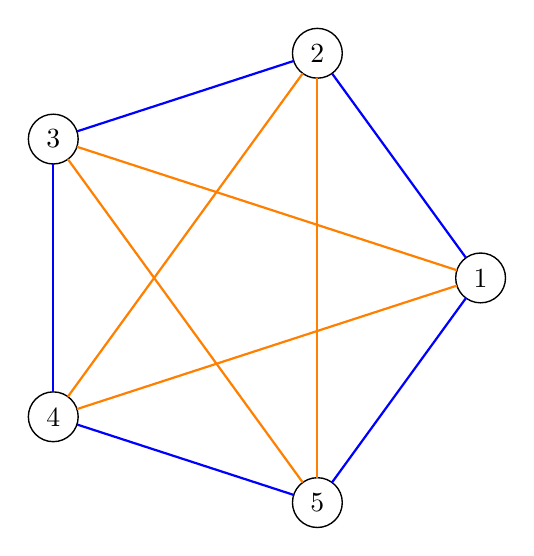
\begin{tikzpicture}
      \SetGraphUnit{3}
      \Vertices{circle}{1, 2, 3, 4, 5}
      \SetUpEdge[color = blue]
      \Edges(1,2,3,4,5,1)
      \SetUpEdge[color = orange]
      \Edges(1,3,5,2,4,1)
    \end{tikzpicture}
  \end{center}
\end{note}

\begin{proposition}[Ramsey theorem for triangles]\index{Ramsey theorem!for triangle}
  Let \(k \in \N\). Then for \(n\) sufficiently large, if \(K_n\) is \(k\)-coloured we must have a monochromatic triangle.
\end{proposition}

\begin{proof}
  Induction on \(k\). For \(k = 1\), \(n = 3\) works. For \(k > 1\), by induction hypothesis we can choose \(m\) such that if \(K_m\) is \((k - 1)\)-coloured then it has a monochromatic triangle. Now take \(n = k(m - 1) + 2\). Suppose \(K_n\) is \(k\)-coloured. Pick \(v \in K_n\). There are \(k(m - 1) + 1\) edges from \(v\) so some \(m\) are the same colour. wlog \(v\) is joint to a \(K_m\), \(H\), by blue edegs. If \(H\) contains a blue edge then we have a blue triangle with \(v\). If not then \(H\) is a \((k - 1)\)-coloured \(K_m\) so by definition of \(m\) it contains a monochromatic triangle.
\end{proof}

\begin{remark}
  How big should we take \(n\)? Write \(f(k)\) for the smallest \(n\) that works. Then \(f(1) = 3\). If \(k > 1\), the proof tells us that \(f(k) \leq k(f(k - 1) - 1) + 2 \leq k f(k - 1)\). So by induction \(f(k) \leq 3k!\).
\end{remark}

\begin{corollary}[Schur's theorem]\index{Schur's theorem}
  Let \(k \geq 1\). Then for \(n\) sufficiently larger, if \([n]\) is partitioned into \(k\) parts we can find \(x, y, z\) in the same part with \(x + y = z\).
\end{corollary}

\begin{proof}
  Let \(n\) be such that if \(K_{n + 1}\) is \(k\)-coloured then there exists a monochromatic triangle. Partition
  \[
    [n] = A_1 \cup \dots \cup A_k.
  \]
  Now \(k\)-colour a \(K_{n + 1}\) with vertices \(0, \dots, n\) using colouring \(c\), with, for \(i < j\), \(j - i \in A_{c(ij)}\). Let \(h < i < j\) be a monochormatic triangle of colour \(u\), say. Then
  \[
    (i - h) + (j - i) = j - h
  \]
  and they are all in \(A_u\).
\end{proof}

We have shown that we can always find a monochromatic triangle, i.e.\ \(K_3\). What about \(K_4, K_5\) etc?

\begin{eg}
  Suppose \(K_{10}\) is coloured blue/yellow. Then there must be a blue triangle or a yellow \(K_4\).

  \begin{proof}
    Pick \(v \in K_{10}\), then
    \begin{itemize}
    \item either \(v\) is in \(4\) blue edges \(vw, vx, vy, vz\). If any edge is among \(w, x, y, z\) is blue, we have a blue triangle. Else \(wxyz\) is a yellow \(K_4\),
      \begin{center}
      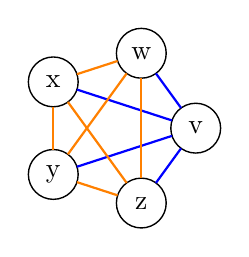
\begin{tikzpicture}
        \Vertices{circle}{v, w, x, y, z}
        \SetUpEdge[color=blue]
        \Edges(w, v, z)
        \Edges(y, v, x)
        \SetUpEdge[color=orange]
        \Edges(w, x, y, z, w, y)
        \Edges(x, z)
      \end{tikzpicture}
      \end{center}
    \item or \(v\) is in \(6\) yellow edges. Let \(H\) be a \(K_6\) joined to \(v\) by yellow edges. We know \(H\) must have a monochromatic triangle. If it is a blue done. Otherwise together with \(v\) we have a yellow \(K_4\).
    \end{itemize}
  \end{proof}
\end{eg}

\begin{definition}[Ramsey number]\index{Ramsey number}
  Let \(s, t \geq 2\). The \emph{Ramsey number} \(R(s, t)\) is the least \(n\) such that whenever \(K_n\) is coloured blue/yellow then we can find a blue \(K_s\) or a yellow \(K_t\) (if such an \(n\) exists). We write \(R(s) = R(s, s)\).
\end{definition}

\begin{theorem}[Ramsey]\index{Ramsey theorem}
  Let \(s, t \geq 2\). Then \(R(s, t)\) exists. Moreover, if \(s, t \geq 3\) then
  \[
    R(s, t) \leq R(s - 1, t) + R(s, t - 1).
  \]
\end{theorem}

\begin{proof}
  Induction on \(s + t\). For \(s = 2\), \(R(2, t) = t\) and similarly for \(t = 2\), \(R(s, 2) = s\). For \(s, t \geq 3\), by induction hypothesis we can take
  \begin{align*}
    m &= R(s - 1, t) \\
    n &= R(s, t -1)
  \end{align*}
  Colour \(K_{m + n}\) blue/yellow. Pick a vertex \(v \in K_{m + n}\). Then
  \begin{itemize}
  \item either \(v\) is in \(m\) blue edges. Let \(H\) be a \(K_m\) joined to \(v\) by blue. By definition of \(m\), \(H\) contains either a blue \(K_{s - 1}\), making a blue \(K_s\) with \(v\) or a yellow \(K_t\).
  \item or \(v\) is in \(n\) yellow edges. Proceed as before with blue/yellow reversed.
  \end{itemize}
  Hence \(R(s, t)\) exists and moreover
  \[
    R(s, t) \leq R(s- 1, t) + R(s, t - 1).
  \]
\end{proof}

How big is \(R(s)\)? We know \(R(2) = 2, R(3) = 6\) so
\[
  R(3, 4) \leq R(3) + R(2, 4) \leq 10.
\]
In fact, in example sheet we will show \(R(3, 4) = 9\). Then
\[
  R(4) = R(4, 4) \leq 2R(3, 4) = 18.
\]
It turns out to be a sharp, which we will also show on example sheet. What about \(R(5)\)? Nobody knows exactly. The bound as the time the note is taken is \(43 \leq R(5) \leq 48\). Although \(5\) seem innocuouly small, the computation required to find the exact Ramsey number is incredibly hard because as \(R(5) \approx 45\), \(K_{45}\) has \(\binom{45}{2} \approx 1000\) edges so there are approximately \(2^{1000}\) blue/yellow colourings.

However, we can easily bound them:

\begin{corollary}
  Let \(s, t \geq 2\). Then \(R(s, t) \leq 2^{s + t}\). In particular, \(R(s) \leq 4^s\).
\end{corollary}

\begin{proof}
  Induction on \(s + t\). For \(s = 2\) have \(R(2, t) = t \leq 2^{2 + t}\). Same for \(t = 2\). For \(s, t \geq 3\),
  \[
    R(s, t) \leq R(s - 1, t) + R(s, t - 1) \leq 2^{s - 1 + t} + 2^{s + t - 1} = 2^{s + t}.
  \]
\end{proof}

\(R(s) \leq 4^s\) seems like a rather crude bound and indeed we start the induction with a very sloppy \(t \leq 2^t\). If we do it more carefully, we get \(R(s, t) \leq \binom{s + t - 2}{s - 1}\) so \(R(s) \leq \binom{2s - 2}{s - 1}\). Approximate, e.g.\ by Stirling formula and we get
\[
  R(s) = O(\frac{4^s}{\sqrt s}),
\]
which is the result by Erdos-Szekeres in 1930s. For 50 years no one is able to improve it. In the 1980s, Andrew Thomason shows \(R(s) = O(\frac{4^s}{s})\), which takes considerably more work. So far the best bound is found by David Conlon in the 2000s, for all \(k\), \(R(s) = O(\frac{4^s}{s^k})\). Is \(R(s) = O((4 - \varepsilon)^s)\) for some \(\varepsilon > 0\)? The answer is unknown.

For a lower bound, however, see example sheet 1.

What if we use more colours? First we can define the Ramsey number correspondingly:

\begin{definition}[multicolour Ramsey number]\index{Ramsey number!multicolour}
  Let \(k \geq 1\) and \(s \geq 2\). The \emph{multicolour Ramsey number} \(R_k(s)\) is the least \(n\) such that whenver \(K_n\) is \(k\)-coloured then there is a monochromatic \(K_s\) (if it exists).
\end{definition}

\begin{theorem}[multicolour Ramsey theorem]\index{Ramsey theorem!multicolour}
  Let \(k \geq 1, s \geq 2\), then \(R_k(s)\) exists.
\end{theorem}

\begin{proof}
  Induction on \(k\). If \(k = 1\) then \(R_1(s) = s\). If \(k = 2\) then \(R_2(s) = R(s)\). For \(k \geq 3\), let \(n = R(s, R_{k - 1}(s))\) which exists by induction hypothesis and Ramsey theorem. Suppose \(K_n\) is \(k\)-coloured, give it now a blue/yellow colouring replacing colour 1 by blue and all others by yellow. Then
  \begin{itemize}
  \item either we have blue \(K_s\), i.e.\ colour 1 \(K_s\).
  \item or yellow \(K_{R_{k - 1}(s)}\). In the original colouring this is \((k - 1)\)-coloured. So we have a monochromatic \(K_s\) inside it.
  \end{itemize}
\end{proof}

\subsubsection{Infinite Ramsey theory}

A short excursion into infinite analogue of Ramsey theorem. Before that we formally define

\begin{definition}[infinite graph]\index{infinite graph}
  An \emph{infinite graph} is an ordered pair \(G = (V, E)\) where \(V\) is an infinite set and \(E\) is a set of unordered pairs of distinct elements of \(V\).
\end{definition}

\begin{note}
  An infinite graph is \emph{not} a graph. This is for the sake of brevity as we will deal mostly with finite graph in this course.
\end{note}

We carry across notations/terminologies from graphs to infinite graphs where possible.

A \emph{not necessarily finite graph} is a graph or an infinite graph.

\begin{definition}
  The \emph{infinite complete graph} \(K_\infty\) is the infinite graph \(K_\infty\) with
  \begin{align*}
    V(K_\infty) &= \N \\
    E(K_\infty) &= \{ij, i, j \in \N, i < j\}.
  \end{align*}
\end{definition}

Suppose we finitely colour \(K_\infty\). What can we find monochromatically? By Ramsey, we get arbitrarily large monochromatic \(K_s\), which is \emph{not} the same as monochormatic \(K_\infty\). For example, we can connect disjoint blue \(K_s\) for \(s \geq 2\) using yellow edges and there is no blue \(K_\infty\). However in this colouring there is a yellow \(K_\infty\).

\begin{theorem}[infinite Ramsey]\index{Ramsey theorem!infinite}
  Let \(K_\infty\) be finitely coloured. Then it contains a monochromatic \(K_\infty\) subgraph.
\end{theorem}

\begin{proof}
  Let \(c: E(K_\infty) \to [k]\) for some \(k\) be a colouring. Pick \(v_1 \in K_\infty\). \(v\) is in infinitely many edges but only finitely many colours so infinitely many of these edges are the same colour. Formally, we can pick an infinite \(A_1 \subseteq V(K_\infty)\) and a colour \(c_1\) such that for all \(w \in A\), \(c(v_1 w) = c_1\).

  Similarly we can pick \(v_2 \in A_1\) and infinite \(A_2 \subseteq A_1\) and colour \(c_2\) such that for all \(w \in A_2\), \(c(v_2w) = c_2\) and so on. We obtain a sequence \(v_1, v_2, \dots, \) of distinct vertices and a sequence \(c_1, c_2, \dots\) of colours and a decreasing sequence \(A_1 \supseteq A_2 \supseteq \dots\) of inifite subsets of \(V(K_\infty)\) such that for all \(i \geq 1\), \(v_{i + 1} \in A_i\) and for all \(w \in A_i\), \(c(v_iw) = c_i\).

  In particular if \(i < j\) then \(c(v_iv_j) = c_i\) so infinitely many of \(c_1, c_2, \dots\) must be the same, say \(n_1 < n_2 < \dots\) with \(c_{n_1} = c_{n_2} = \dots\). Now let \(H\) be the infinite complete subgraph with vertex set \(\{v_{n_i}: i \geq 1\}\). Suppose \(i < j\). Then \(n_i < n_j\) and so \(c(v_{n_i}v_{n_j}) = c_{n_i} = c_{n_1}\). Thus \(H\) is monochromatic.
\end{proof}

\begin{remark}
  This is sometimes called a ``two-pass proof''.
\end{remark}

As a byproduct we have

\begin{corollary}[Bolzano-Weierstrass]
  A bounded real sequence has a convergent subsequence.
\end{corollary}

\begin{proof}
  Any bounded monotone sequence converges so enough to show if \((x_n)\) is a real sequence then it must have a monotone subsequence.

  Let \(G\) be \(K_\infty\) with vertex set \(\N\). Colour \(G\) blue/yellow by giving \(ij, i < j\) colour blue if \(x_i < x_j\) or yellow if \(x_i \geq x_j\). By infinite Ramsey theorem we have in infinite monochromatic complete subgraph \(H\), say with vertices \(n_1 < n_2 < \dots\). Consider the subsequence \((x_{n_j})\). If \(H\) is blue then \((x_{n_j})\) is (strictly increasing), while if \(H\) yellow then \((x_{n_j})\) is decreasing.
\end{proof}

\subsection{Basic definitions and concepts}

\begin{eg}
  Some examples of graphs:
  \begin{enumerate}
  \item Complete graph of order \(n\): \(K_n\) with \(V(K_n) = [n], E(K_n) = \{ij: 1 \leq i < j \leq n\}\).
  \item Path of length \(n\): \(P_n\) with \(V(P_n) = \{0, \dots, n\}, E(P_n) = \{i(i + 1): 0 \leq i < n\}\).
  \item Cycle of length \(n\): \(C_n\) with \(V(C_n) = [n], E(C_n) = \{i(i + 1): 1 \leq i < n\} \cup \{n1\}\).
  \end{enumerate}
\end{eg}

\begin{definition}[order]\index{order}
  Let \(G = (V, E)\) be a graph. The \emph{order} of \(G\) is \(|G| = |V|\).

  We also write \(e(G) = |E|\). (sometimes call the \emph{size} of \(G\))
\end{definition}

\begin{eg}\leavevmode
  \begin{enumerate}
  \item \(|K_n| = n, e(K_n) = \binom{n}{2}\).
  \item \(|P_n| = n + 1, e(P_n) = n\).
  \item \(|C_n| = n, e(C_n) = n\).
  \end{enumerate}
\end{eg}

\begin{definition}[spanned subgraph]\index{subgraph!spanned}
  Suppose \(G = (V, E)\) is a graph and \(U \subseteq V\). The subgraph of \(G\) \emph{spanned} or \emph{induced} by \(U\) is the subgraph \(G[U]\) of \(G\) with \(V(G[U]) = U, E(G[U]) = \{ij \in E: i, j \in U\}\).
\end{definition}

\begin{definition}[disjoint union]
  Suppose \(G = (V, E), G' = (V', E')\) are graphs with \(V \cap V' = \emptyset\). The \emph{disjoint union} of \(G, G'\) is the graph \(G \cup G' = (V \cup V', E \cup E')\).
\end{definition}

Sometimes we use this terminology more loosely, when \(V\) and \(V'\) are not disjoint, to mean ``take isomorphic copies of \(G\) and \(G'\) with disjoint vertex sets and form their disjoint union''.

\begin{eg}
  \(C_5 \cup P_3\) (graph)
  \iffalse
  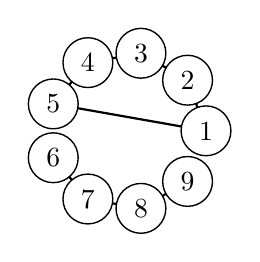
\begin{tikzpicture}
    \Vertices{circle}{1, 2, 3, 4, 5, 6, 7, 8, 9}
    \Edges(1, 2, 3, 4, 5, 1)
    \Edges(6, 7, 8, 9)
  \end{tikzpicture}
  \fi
\end{eg}

We need a bit more notations/definitions. Let \(G = (V, E)\) be a graph. If \(U \subseteq V\), the graph \(G - U\) is defined to be \(G - U = G[V \setminus U]\). If \(U = \{v\}\), write \(G - v = G - U\).

If \(F \subseteq E\), write \(G - F = (V, E \setminus F)\). If \(F = \{e\}\), write \(G - e = G - F\).

The \emph{complement}\index{complement} of \(G\) is the graph \(\overline G\) with
\begin{align*}
  V(\overline G) &= G \\
  E(\overline G) &= \{uv: u, v \in V, u \neq v, uv \neq E\}
\end{align*}

\begin{eg}\leavevmode
  \begin{enumerate}
  \item The complement of the complement graph \(K_n\) is the \emph{empty graph} of order \(n\), \(\overline K_n\), with \(n\) vertices and no edges.
  \item The complement of \(C_5\) is
    \begin{center}
    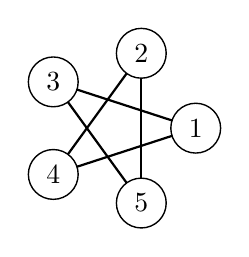
\begin{tikzpicture}
      \Vertices{circle}{1, 2, 3, 4, 5}
      \Edges(1, 3, 5, 2, 4, 1)
    \end{tikzpicture}
    \end{center}
    which is isomorphic to \(C_5\). We say \(C_5\) is \emph{self-complementary}.
  \end{enumerate}
\end{eg}

We say \(v, w \in G\) are \emph{adjacent}\index{adjacent} or \emph{neighbours} and write \(v \sim w\) if \(vw \in E\). The \emph{neighbourhodd} of \(v\) is
\[
  \Gamma(v) = \{w \in G: v \sim w\}.
\]
The \emph{degree}\index{degree} of \(v\) is the number of neighbours of \(v\): \(d(v) = |\Gamma(v)|\). More generally, if \(A \subseteq V\), the \emph{neighbourhood}\index{neighbourhood} of \(A\) is
\[
  \Gamma(A) = \bigcup_{v \in A} \Gamma(v).
\]
The \emph{minimum degree} of \(G\) is \(\delta(G) = \min_{v \in G} d(v)\). The \emph{maximum degree} of \(G\) is \(\Delta(G) = \max_{v \in G} d(v)\). The \emph{average degree} of \(G\) is
\[
  \overline d (G) = \frac{1}{|G|} \sum_{v \in G} d(v).
\]

Observe that
\begin{enumerate}
\item \(\delta(G) \leq \overline d(G) \leq \Delta(G)\). If either, i.e.\ both, are equalities we say \(G\) is \emph{regular}\index{graph!regular}. If \(G\) is regular, all vertices have the same degree. If that degree is \(r\), we say \(G\) is \emph{\(r\)-regular}.
\begin{eg}
  \(K_n\) is \((n - 1)\)-regular. \(\overline K_n\) is \(0\)-regular. \(C_n\) is \(2\)-regular. \(P_n\) is not regular for \(n \geq 2\) as \(\delta(P_n) = 1\) and \(\Delta(P_n) = 2\).
\end{eg}
\item \(2 e(G) = \sum_{v \in G} d(v)\). It is obvious as an edge has two ``ends''. A formal proof: let
  \[
    X = \{(e, v): e \in E, v \in e\}.
  \]
  To pick \((e, v) \in X\), we can choose \(e\) in \(e(G)\) ways then we choices for \(v\). So \(|X| = e(G) \times 2\). Alternatively, pick \(v\) first then, given \(v\), \(d(v)\) choices from \(e\) so \(|X| = \sum_{v\in G} d(v)\).

  This gives \(e(G) = \frac{|G| \overline d(G)}{2}\).
\end{enumerate}

A \emph{path}\index{path} in \(G\) from \(v\) to \(w\) where \(v, w \in G\), is a sequence \(v_0, v_1, \dots, v_\ell\) of distinct vertices of \(G\) where \(v_0 = v, v_\ell = w\) and \(v_{i - 1} \sim v_i\) for \(1 \leq i \leq \ell\). Usually write this path as \(v_0v_1\dots v_\ell\). The \emph{length}\index{length} of the path is \(\ell\). A path of length \(\ell\) in \(G\) yields a subgraph isomorphic to \(P_\ell\). In particular \(v\) is a path (of length \(0\)) from \(v\) to \(v\).

Define a relation \(\to\) on \(V(G)\) by \(v \to w\) if there is a path from \(v\) to \(w\). It is an equivalence relation (example sheet 2). The equivalence class of \(\to\) are the \emph{connected componenets}\index{connected componenets} of \(G\). Note \(G\) is the disjoint union of its components. If \(G\) has only one component, we say \(G\) is \emph{connected}\index{graph!connected}.

\begin{eg}
  A graph with three components (graph)
\end{eg}

A \emph{cycle of length \(n\)} in \(G\) is a subgraph of \(G\) isomorphic to \(C_n\). Often denote such by \(v_1v_2\dots v_nv_1\) where \(v_1, \dots v_n \in v(G)\) are distinct, \(v_{i - 1} \sim v_n\) for \(1 < i \leq n\) and \(v_n \sim v_1\). Note that unlike path, cycle does not have a starting point or direction. Thus there are many notations for some cycles, for example \(abcdea = dcbaed\).

A final notation: we often write \(e \in G\) to mean \(e \in E(G)\) if unambiguous.

\subsubsection{Bipartite graphs}

\begin{definition}[bipartite graph]\index{bipartite graph}
  A graph \(G = (V, E)\) is \emph{bipartite} if there is a partition \(V = X \cup Y\) such that any \(e \in E\) can be written \(e = xy\) where \(x \in X\), \(y \in Y\).

  The \emph{complete bipartite graph} \(K_{m, n}\) has \(|X| = m, |Y| = n\) and \(xy \in E(K_{m, n})\) for all \(x \in X, y \in Y\).
\end{definition}

\begin{eg}
  \(K_{2, 3}\)
  \iffalse
  \begin{center}
    \begin{tikzpicture}
      \Vertices{1, 2}
    \end{tikzpicture}
  \end{center}
  \fi
\end{eg}

In general, \(|K_{m, n}| = m + n, e(K_{m, n}) = mn\). There is a more useful characterisation of bipartite graphs:

\begin{proposition}
  A graph \(G = (V, E)\) is bipartite if and only if it contains no odd cycles.
\end{proposition}

\begin{proof}
  Suppose \(G = (V, E)\) is bipartite and \(V = X \cup Y\) is a partition. Assume for contradiction \(v_1v_2 \dots v_nv_1\) is a cycle with \(n\) odd. wlog \(v_1 \in X\). Then \(v_2 \in Y, v_2 \in X, \dots, v_n \in X, v_1 \in Y\). Contradiction.

  Suppose \(G\) has no odd cycles. wlog \(G\) is connected. Pick \(x \in G\). For \(y \in G\), define the distance from \(x\) to \(y\), \(d(x, y)\) to be the shortest path from \(x\) to \(y\). Let
  \[
    V_i = \{y \in G: d(x, y) = i\}
  \]
  for \(i \geq 0\). Let \(X = \bigcup_{i \text{ even}} V_i, Y = \bigcup_{i \text{ odd}} V_i\). Let \(uv \in E(G)\) with \(u \in V_j, v \in V_k\) where \(j \leq k\). Then must have \(k = j\) or \(k = j + 1\). Indeed there is a path of length \(j + 1\) from \(x\) to \(v\). 

  Suppose \(k = j\). We want to say that \(x, u\) and \(v\) form a cycle of length \(2j + 1\), but they may intersect somewhere earlier in the path. The standard way to deal with it is to take the closest intersection. Let \(u_0u_1 \dots u_j\) and \(v_0v_1 \dots v_j\) be shortest paths from \(x\) to \(u\) and \(v\) respectively, so \(u_0 = v_0 = x\), \(u_j = u\), \(v_j = v\) and \(u_i, v_i \in V_i\) for \(0 \leq i \leq j\). In particular, \(h \neq i\) implies that \(u_h \neq v_i\). Pick \(i\) largest such that \(u_i = v_i\), so \(0 \leq i < j\) and \(u_iu_{i + 1} \dots u_j v_j \dots v_i\) is a cycle of length \(2(j - i) + 1\) which is odd.
\end{proof}

\subsection{The forbidden subgraph problem}

\subsubsection{Complete subgraphs}

The problem of determining \(R(s)\) can be thought of as ``how many vertices can \(G\) have yet \(K_s \nsubseteq G\) and \(K_s \nsubseteq \overline G\). This is a typical example of an \emph{extremal problem}: how large can some parameter of a graph be before the graph is forced to have a certain property?

\begin{eg}
  Let \(|G| = n\). How large can \(e(G)\) get before \(G\) is forced to contain a triangle?
\end{eg}

The idea is to try \(G\) bipartite, as we know bipartite graphs do not contain triangles. Clearly we need complete bipartite graph so seek \(K_{s, t}\) where \(s + t = n\) so that \(E(K_{s, t}) = st = s(n - s)\) is maximised. This is achieved when \(s = \frac{n}{2}\) when \(n\) is even or \(s = \frac{n \pm 1}{2}\) when \(s\) is odd. Among bipartite graphs, \(K_{\floor{n/2}, \ceil{n/2}}\) is the best. Can we do better?

Adding any edge to it creates a triangle but this isn't enough. For example, \(C_5\) is not bipartite but has the same property but clearly it isn't the best.
\begin{center}
  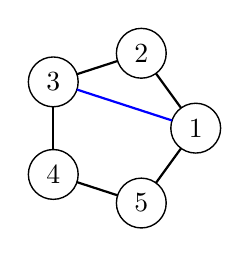
\begin{tikzpicture}
    \SetUpEdge[color = black]
    \Vertices{circle}{1, 2, 3, 4, 5}
    \Edges(1, 2, 3, 4, 5, 1)
    \SetUpEdge[color = blue]
    \Edges(1, 3)
  \end{tikzpicture}
\end{center}

In fact, bipartite always wins but we need to do some work.

\begin{proposition}[Mantel's theorem]\index{Mantel's theorem}
  Let \(|G| = n \geq 3, e(G) \geq \floor{\frac{n^2}{4}}\) and \(\triangle \nsubseteq G\). Then
  \[
    G \cong K_{\floor{n/2}, \ceil{n/2}}.
  \]
\end{proposition}

\begin{remark}
  It follows immediately that if \(|G| = n, e(G) > \floor{\frac{n^2}{4}}\) and \(\triangle \nsubseteq G\) then it is isomorphic to \(K_{\floor{n/2}, \ceil{n/2}}\) so \(e(G) = \floor{\frac{n^2}{4}}\), absurd. Thus \(K_{\floor{n/2}, \ceil{n/2}}\) has the most edges for a \(\triangle\)-free graph. The theorem asserts something stronger: it is \emph{uniquely} the best up to isomorphism.
\end{remark}

\begin{proof}
  Induction on \(n\). For \(n = 3\), \(|G| = 3, e(G) \geq 2, \triangle \nsubseteq G\) then \(G \cong K_{1, 2}\). For \(n \geq 4\), assume for now \(n\) is even so \(|G| = n, e(G) \geq \frac{n^2}{4}\), \(\triangle \nsubseteq G\). First delete edges from \(G\) if necessary to obtain a graph \(H\) with \(|H| = n, e(H) = \frac{n^2}{4}, \triangle \nsubseteq H\). Next pick \(v \in H\) of minimum degree and \(K = H - v\). Then \(|K| = n - 1\) and \(\triangle \nsubseteq K\). To bound \(e(K)\), note that
  \[
    d(v) = \delta(H) \leq \overline d(H) = \frac{1}{|H|} \sum_{x \in H} d(x)
    = \frac{1}{|H|} 2 e(H)
    = \frac{1}{n} \cdot 2 \frac{n^2}{4}
    = \frac{n}{2}
  \]
  so
  \[
    e(K) = e(H) - d(v)
    \geq \frac{n^2}{4} - \frac{n}{2}
    = \frac{(n - 1)^2}{4} - \frac{1}{4}
    = \floor*{\frac{(n - 1)^2}{4}}
  \]
  so by induction hypothesis
  \[
    K \cong K_{\floor{(n - 1)/2}, \ceil{(n - 1)/2}} = K_{\frac{n}{2} - 1, \frac{n}{2}}.
  \]
  To recover \(H\), we should add a vertex \(v\) to \(K\), joining it to precisely \(\frac{n}{2}\) vertices of \(K\) but creating no triangle. The only way to do this is to join \(v\) to all \(\ceil{\frac{n}{2}}\) vertices in one partition of \(K\). This thus gives \(H \cong K_{n/2, n/2}\).

  Finally \(G\) can be recovered by adding edges to \(H\) without making \(\triangle\). But this is impossible so \(G = H\), i.e.\ we did not in fact delete any edges in the beginning.

  \(n \geq 4\), \(n\) odd is similar.
\end{proof}

What about forbidding \(K_4\)? Should we try ``tripartite'' graphs?

\begin{definition}[\(r\)-partite]\index{graph!\(r\)-partite}
  A graph \(G\) is \emph{\(r\)-partite} if we can partition if \(V(G) = X_1 \cup X_2 \cup \dots \cup X_r\) such that \(u,v \in X_i\) for some \(i\) then \(u \nsim v\).

  It is \emph{complete \(r\)-partite} if \(u \in X_i, v \in X_j\) for \(i \neq j\) implies \(u \sim v\).
\end{definition}

Which \(r\)-bipartite graph of order \(n\) has most edges? Obviously such a \(G\) is complete \(r\)-bipartite. Suppose \(G\) has some two vertex classes \(X, Y\) with \(|X| \geq |Y| + 2\). Move a vertex \(v\) from \(X\) to \(Y\). We gain \(|X| - 1\) edges and lose \(|Y|\) edges. The net gain is \(|X| - 1 - |Y| \geq 1\), contradiction.

\begin{definition}[Turán graph]\index{Turán graph}
  The \emph{Turán graph} \(T_r(n)\) is the complete \(r\)-partite graph of order \(n\) with vertex classes as equal as possible. We write \(t_r(n) = e(T_r(n))\).
\end{definition}

\begin{eg}
  \(T_2(n) = K_{\floor{n/2}, \ceil{n/2}}\) and \(t_2(n) = \floor*{\frac{n^2}{4}}\). Mantel's theorem can be rephrased as to get most edges with no \(K_3\), take \(T_2(n)\).
\end{eg}

Some properties of Turán graphs:
\begin{enumerate}
\item \(K_{r + 1} \nsubseteq T_r(n)\) but adding any edge to \(T_r(n)\) makes a \(K_{r + 1}\).
\item If \(r \divides n\) then all vertex classes are the same size, namely \(\frac{n}{r}\). If \(r \ndivides n\), we have some small classes with \(\floor*{\frac{n}{r}}\) vertices and some large classes with \(\ceil*{\frac{n}{r}} = \floor*{\frac{n}{r}} + 1\) vertices
\item Each vertex is joined to everyting except vertices in its own class. Therefore if \(r \divides n\) then \(T_r(n)\) is regular. If \(r \ndivides n\) then \(v \in T_r(n)\) in a large class has \(d(v) = \delta(T_r(n))\) whereas if \(v\) is in a small class, \(d(v) = \Delta(T_r(n)) = \delta(T_r(n)) + 1\). Hence in either case, give the order and average degree, the vertex degrees are as equal as possible.
\item What happens if we delete \(v \in T_r(n)\) of minimum degree? Then \(v\) is in a large class so we get \(T_r(n - 1)\). Therefore
  \[
    t_r(n) - \delta(T_r(n)) = t_r(n - 1).
  \]
\item Suppose we want to add a vertex \(v\) to \(T_r(n - 1)\) of as large degree as possible without making a \(K_{r + 1}\). We can't join \(v\) to a vertex in every class. So best is to join \(v\) to everything except a small class. This makes \(T_r(n)\). The biggest degree we can achieve for \(v\) is \(t_r(n) - t_r(n - 1)\) and only way to do this is to make \(T_r(n)\).
\end{enumerate}

\begin{theorem}[Turán]\index{Turán's theorem}
  Let \(|G| = n, e(G) \geq t_r(n)\) and \(K_{r + 1} \nsubseteq G\) (\(n \geq r + 1 \geq 3\)). Then \(G \cong T_r(n)\).
\end{theorem}

Note that Mantel's theorem is just a special case with \(r = 2\).

\begin{proof}
  Induction on \(n\). Suppose \(n = r + 1\). \(T_r(r + 1)\) has one class with two vertices and all other classes with one vertex, so \(T_r(r + 1)\) is \(K_{r + 1}\) minus an edge. For \(n > r + 1\), if necessary, delete edges from \(G\) to obtain \(H\) with \(|H| = n, e(H) = t_r(n)\) and \(K_{r + 1} \nsubseteq H\). Pick \(v \in H\) of minimum degree and let \(K = H - v\). Then \(|K| = n - 1\) and \(K_{r + 1} \nsubseteq K\). We know \(|H| = |T_r(n)|\) and \(e(H) = e(T_r(n))\) so
  \[
    \overline d(H) = \overline d(T_r(n)).
  \]
  But in \(T_r(n)\) vertex degrees are as equal as possible. Hence
  \[
    \delta(H) \leq \delta(T_r(n))
  \]
  and hence
  \[
    e(K) = e(H) - \delta(H) \geq t_r(n) - \delta(T_r(n)) = t_r(n - 1)
  \]
  so by induction hypothesis, \(K \cong T_r(n - 1)\). To recover \(H\) we need to add \(v\) to \(K\) of degree \(e(H) - e(K) = t_r(n) - t_r(n - 1)\) without making a \(K_{r + 1}\). So \(H \cong T_r(n)\). Adding an edge to \(H\) makes a \(K_{r + 1}\) so \(G = H \cong T_r(n)\).
\end{proof}

This is a special case of the \emph{forbidden subgraph problem}\index{forbidden subgraph problem}: fix a graph \(H\) with at least one edge. How many edges can a graph \(G\) of order \(n\) have yet not contain \(H\) as a subgraph?

Write
\[
  \exx(n; H) = \max \{e(G): |G| = n, H \nsubseteq G\},
\]
then Turán's theorem can be stated as \(\exx(n, K_{r + 1}) = t_r(n)\).

\subsubsection{Complete bipartite subgraphs}

What is \(\exx(n; C_4)\)? Suppose we have \(|G| = n, e(G) = m\) and \(C_4 \nsubseteq G\). How large can \(m\) be? The idea is to count the number of \(P_2\)-subgraphs, \(A\), in \(G\) in two different ways. Each \(v \in G\) is the middle vertex of \(\binom{d(v)}{2}\) \(P_2\)'s so
\[
  A = \sum_{v \in G} \binom{d(v)}{2}.
\]
Alternatively, as \(C_4 \nsubseteq G\), each pair of vertices are the end-vertices of at most one \(P_2\). (graph) so
\[
  A \leq \binom{n}{2}.
\]
It gives a bound on \(n\)
\[
  \binom{n}{2} \geq \sum_{v \in G} \binom{d(v)}{2}.
\]
The function \(x \mapsto \binom{x}{2}\) is convex so, writing \(\frac{m}{n} = a\),
\[
  \binom{n}{2} \geq \sum_{v \in G} \binom{d(v)}{2}
  \geq n \binom{\frac{1}{n} \sum_{v \in G} d(v)}{2}
  = n \binom{\frac{2m}{n}}{2}
  = n \binom{2a}{2}
\]
so
\[
  \frac{n(n - 1)}{2} \geq \frac{n 2a (2 a - 1)}{2}.
\]
Rearrange to get
\[
  4a^2 - 2a - (n - 1) \leq 0
\]
so
\[
  a \leq \frac{2 + \sqrt{4 + 16 (n - 1)}}{8} = \frac{1}{4}(1 + \sqrt{4n - 3})
\]
so
\[
  m \leq \frac{n}{4} (1 + \sqrt{4n - 3})
\]
and \(\exx(n; C_4) = O(n \sqrt n)\).

This is a fairly typical for extremal problesm --- usually we don't get exact answer but get some sort of bounds/aymptotics.

\begin{remark}\leavevmode
  \begin{enumerate}
  \item Note that we used \emph{Jensen's inequality}: let \(f: I \to \R\) be convex where \(I\) is an interval and \(x_1, \dots x_n \in I\). Then
    \[
      \frac{1}{n} \sum_{i = 1}^n f(x) \geq f(\frac{1}{n} \sum_{i = 1}^n x_i).
    \]
  \item Also a quick remark about binomial coefficients: if \(x \in \R\) and \(a \geq 0\) integer, we define
    \[
      \binom{x}{a} = \frac{x (x - 1) \dots (x - a + 1)}{a!}.
    \]
    Standard bounds:
    \[
      \binom{x}{a} \leq \frac{x^a}{a!}
    \]
    as long as \(x \geq a - 1\). On the other hand,
    \[
      \binom{x}{a} \geq \frac{(x - a + 1)^a}{a!} \geq \frac{1}{a!} \left(\frac{x}{2} \right)^a
    \]
    as long as \(x \geq 2 (a - 1)\). Usually when dealing with extremal graph problems, we suppose the parameters are sufficeintly large so these bounds apply.
  \item Note \(x \mapsto \binom{x}{2}\) is convex on \(\R\) but \(x \mapsto \binom{x}{a}\) is not. However, it is convex on \([a - 1, \infty)\), by writing \(y = x - a + 1\) to get a polynomial with positive coefficients.
  \end{enumerate}
\end{remark}

Let's got for \(\exx(n; K_{t, t})\) for \(t \geq 2\). We shall count \(t\)-fans (graph). In particular a \(2\)-fan is a \(P_2\) subgraph.

\begin{definition}[fan]\index{fan}
  A \emph{\(t\)-fan} in a graph \(G\) is an ordered pair \((v, U)\) where \(v \in G, U \subseteq V(G), |U| = t\) and for all \(u \in U, v \sim u\).
\end{definition}

\begin{theorem}
  Let \(t \geq 2\). Then
  \[
    \exx(n, K_{t, t}) = O(n^{2 - \frac{1}{t}}).
  \]
\end{theorem}

\begin{proof}
  Let \(|G| = n, e(G) = m, K_{t, t} \nsubseteq G\). Let \(A\) be the number of \(t\)-fans in \(G\). To pick a \(t\)-fan \((v, U)\), can choose \(v \in G\) then \(U \subseteq \Gamma(v)\) with \(|U| = t\) so
  \[
    A = \sum_{v \in G} \binom{d(v)}{t}.
  \]
  As \(K_{t, t} \nsubseteq G\), for any \(U \subseteq V(G)\) with \(|U| = t\), there are at most \((t - 1)\) \(t\)-fans of the form \((v, U)\). So
  \[
    A \leq (t - 1) \binom{n}{t}.
  \]
  Technically we are done. To extract the explicit bound,
  \begin{align*}
    (t - 1) \frac{n^t}{t!}
    &\geq (t - 1) \binom{n}{t} \\
    &\geq A \\
    &= \sum_{v \in G} \binom{d(v)}{t} \\
    &\geq n \binom{\frac{1}{n} \sum_{v \in G} d(v)}{t} \\
    &= n \binom{\frac{2m}{n}}{t} \\
    &\geq \frac{n}{t!} \left(\frac{m}{n}\right)^t
  \end{align*}
  assuming \(\frac{m}{n}\) is sufficiently large. Hence
  \[
    \left( \frac{m}{n} \right)^t \leq (t - 1) n^{t - 1}
  \]
  and so
  \[
    m \leq (t - 1)^{\frac{1}{t}} n^{2 - \frac{1}{t}}.
  \]
\end{proof}

\begin{remark}\leavevmode
  \begin{enumerate}
  \item Why can we assume that \(\frac{m}{n}\) is sufficiently large? For lower bound on binomial coefficient, we need \(\frac{2m}{n} \geq 2(t - 1)\), i.e.\ \(m \geq (t - 1) n\). If not true then \(m < (t - 1)n\) so we don't care. Technically, we're really showing
    \[
      m < \max\{(t - 1)n , (t - 1)^{\frac{1}{t}} n^{2 - \frac{1}{t}} = O(n^{2 - \frac{1}{t}})\}.
    \]
  \item Can we use Jensen's inequality? We know \(x \mapsto \binom{x}{t}\) is convex on \([t - 1, \infty)\) and \(\binom{t - 1}{t} = 0\). Also we know if \(d(v) < t - 1\) then \(\binom{d(v)}{t} = 0\) so really we are apply Jensen's inequality to
    \[
      f(x) =
      \begin{cases}
        0 & x < t - 1 \\
        \binom{x}{t} & x \geq t - 1
      \end{cases}
    \]
    which is clearly convex. As \(\frac{m}{n}\) sufficiently large, \(\frac{2m}{n} \geq t - 1\) so \(f(\frac{2m}{n} = \binom{2m/n}{t}\).
\item This is closely related to the \emph{problem of Zarankiewicz}: we define
  \[
    Z(n, r) = \max \{e(G): \text{ \(G\) bipartite, \(n\) vertices in each class, \(K_{t, t} \nsubseteq G\)}\},
  \]
  the \emph{Zarankiewicz number}.
  \end{enumerate}
\end{remark}

\begin{corollary}
  Let \(t \geq 2\). Then
  \[
    Z(n, t) = O(n^{2 - \frac{1}{t}}).
  \]
\end{corollary}

\begin{proof}
  \[
    Z(n, t) \leq \exx(2n, K_{t, t}).
  \]
\end{proof}

\subsection{General subgraphs}

Let \(H\) be any graph with at least one dege. What is \(\exx(n; H)\)? It is too much to hope for exact results so we aim to find asymptotics. Consider, say,
\[
  \frac{\exx(n; H)}{\binom{n}{2}},
\]
``the proportion of edges of an \(H\)-free graph can have''. What happens as \(n \to \infty\)? If this converges, let
\[
  \exx(H) := \lim_{n \to \infty} \frac{\exx(n; H)}{\binom{n}{2}}.
\]

\begin{eg}\leavevmode
  \begin{enumerate}
  \item Turán: \(\exx(n, K_{r + 1}) = t_r(n) \approx (1 - \frac{1}{r}) \binom{n}{2}\). In fact \(\exx(K_{r + 1}) = 1 - \frac{1}{r}\).
  \item \(\exx(n, K_{t, t}) = O(n^{2 - \frac{1}{t}}) = o(n^2)\) so \(\exx(K_{t, t}) = 0\).
  \item For \(H\) any bipartite graph with at least one edge. Then \(H \subseteq K_{t, t}\) for some \(t\) so \(K_{t, t} \subseteq G\) implies that \(H \subseteq G\) so for all \(n\),
    \[
      \exx(n; H) \leq \exx(n; K_{t, t})
    \]
    so \(\exx(H) = 0\).
  \end{enumerate}
\end{eg}









\iffalse
% 2017 lecture

Revision of \(\bigO\) notation and its cousins: let \(f,g:\N\to (0,\infty)\). We say
\begin{align*}
  f &= \bigO(g) \text{ if } f< Ag \text{ for some constant } A \\
  f &= \Omg(g) \text{ if } g=\bigO(f) \\
  f &= \bigT(g) \text{ if } f=\bigO(g) \text{ and } f = \Omg(g).
\end{align*}
Also,
\begin{align*}
  f &= \smallo(g) \text{ if } f/g\to 0 \text{ as } n\to \infty \\
  f &= \smallomg(g) \text{ if } f/g\to \infty \\
  f &\sim g \text{ if } f/g\to 1.
\end{align*}



\begin{question}
  How large must \(n\) be so that if edges of \(K_n\) are coloured blue and yellow then we always get mono \(K_s\)?
\end{question}

Let \(G\) be ``blue subgraph'' of \(K_n\), i.e. all vertices, only blue edges.
\begin{align*}
  K_n \text{ has a blue } K_s &\Leftrightarrow K_s \subseteq G \\
  K_n \text{ has a yellow } K_s &\Leftrightarrow G \text{ has an induced } \stcomp{K_s} \text{ subgraph}
\end{align*}

Rephrase: how large must \(n\) be to force every graph of order \(n\) to have \(K_s\) or \(\stcomp{K_s}\) as an induced subgraph?

This is a typical example of an \emph{extremal problem}: how large must some parameter of \(G\) be to force \(G\) to have a certain property?

Alternatively, how big can the parameter be with \(G\) not having the property?

\subsection{The Forbidden Subgraph Problem}

Fix a graph \(H\) with at least one edge. Let \(n \geq |H|\). Clearly \(H \subseteq K_n\) but \(H \nsubseteq \stcomp{K_n}\). How many edges must a graph \(G\) of order \(n\) have to force \(H \subseteq G\)? Alternatively, if \(|G| = n\) and \(H \nsubseteq G\), how large can \(e(G)\) be?

\begin{definition}
  Define
  \[
    \exx(n,H) := \max\{ e(G): |G|=n, H \nsubseteq G\}.
  \]
\end{definition}

\begin{question}
  Can we determine \(\exx(n,H)\)?
\end{question}

\subsubsection{Triangles}

Let \(H = K_3\). Want \(G\) with \(|G| = n\), \(e(G)\) large, \(\triangle \nsubseteq G\). Try partitioning \(V(G) = X\cup Y\) with all edges going from \(X\) to \(Y\).

\begin{definition}[Bipartite graph]
  A graph \(G\) is \emph{bipartite} (with bipartition \((X,Y)\)) if \(V(G)\) can be partitioned as \(X\cup Y\) in such a way that if \(e\in E(G)\) then \(e=xy\) for some \(x\in X, y\in Y\).
\end{definition}

Bipartite graphs have no \(\triangle\) (and indeed no cycles of odd length). In fact, the converse if true:

\begin{theorem}
  A graph is bipartite if and only if it contain no odd cycles.
\end{theorem}

\begin{proof}
  Later. Or exercise if you're ambitious.
\end{proof}

\begin{question}
  Which bipartite graph is the best?
\end{question}

Clearly want to include all possible edges from \(X\) to \(Y\).

\begin{definition}[Complete bipartite graph]
  Let \(s,t\geq 1\). The \emph{complete bipartite graph} \(K_{s,t}\) has bipartition \((X,Y)\) with \(|X| = s, |Y| = t\) and \(xy \in E(K_{s,t})\) for all \(x\in X, y\in Y\).
\end{definition}

We have
\begin{align*}
  |K_{s,t}| &= s+t \\
  e(K_{s,t}) &= st
\end{align*}
We want to maximise \(st\) subject to \(s+t=n\), i.e. maximise \(s(n-s)\), which is a quadratic in \(s\). So the best bipartite graph is
\[
  K_{\floor*{\frac{n}{2}}, \ceil*{\frac{n}{2}}}.
\]
But what if some \emph{non-bipartite} graph is better? For example, \(G\) is not bipartite but \(\triangle \nsubseteq G\) so \(e(K_{3,2}) = 6 > 5 = e(G)\). It turns out we don't have to worry: bipartite graph always wins.

\begin{theorem}[Mantel's Theorem]
  Let \(n\geq 3\). Suppose \(|G| = n, e(G) \geq \floor*{\frac{n^2}{4}}\) and \(\triangle \nsubseteq G\). Then
  \[
    G \cong K_{\floor*{\frac{n}{2}}, \ceil*{\frac{n}{2}}}.
  \]
\end{theorem}

\begin{proof}
  Proceed by induction on \(n\): if \(n=3\), there is only one possibility: \(G = K_{2,1}\). For \(n>3\), first remove edges from \(G\) if necessary to get \(H\) with \(|H| = n, e(H) = \floor*{\frac{n^2}{4}}\). Clearly \(\triangle \nsubseteq H\). Let \(v\in H\) with \(d(v) = \delta(H)\) and let \(K = H-v\). In other words, \(H\) with vertex \(v\) and all edges including \(v\) removed. Now \(|K| = n-1, \triangle \nsubseteq K\) and \(e(K) = \floor*{\frac{n^2}{4}} - \delta(H)\).

  Suppose \(n\) is even. Then
  \[
    \delta(H) \leq \text{average degree of } H = \frac{2e(H)}{|H|} = \frac{n^2/2}{n} = \frac{n}{2}.
  \]
  Hence \(e(K) \geq \frac{n^2}{4} - \frac{n}{2} = \frac{(n-1)^2}{4}-\frac{1}{4} = \floor*{\frac{(n-1)^2}{4}}\).

  Similarly if \(n\) is odd, also get \(e(K) \geq \floor*{\frac{(n-1)^2}{4}}\). Hence by induction hypothesis
  \[
    K \cong K_{\frac{n-1}{2},\frac{n-1}{2}}
  \]

  Also \(d(v) = e(H) - e(K)\) so if \(n\) is even
  \[
    d(v) = \frac{n^2}{4} - \frac{n^2-2n}{4} = \frac{n}{2}.
  \]
  \(H\) is formed by adding a vertex \(v\) to \(K \cong K_{\frac{n}{2},\frac{n-2}{2}}\), and joining \(v\) to \(\frac{n}{2}\) vertices of \(K_1\) without creating a \(\triangle\). If \(K\) has biparition \((X,Y)\), \(v\) cannot be joined both to vertex in \(X\) and vertex in \(Y\) so \(v\) must be joined to all vertices in larger of \(X\) and \(Y\). Thus \(H \cong K_{\floor*{\frac{n}{2}},\ceil*{\frac{n}{2}}}\) (and similar if \(n\) is odd).

  We recover \(G\) by adding edges to \(H\) without making a \(\triangle\). But any new edge creates a \(\triangle\). So \(G \cong H\).
\end{proof}

Hence if \(|G|=n, e(G) > floor \frac{n^2}{4}\) then \(G\) contains a \(\triangle\). Therefore \(\exx(n, \triangle) = \floor*{\frac{n^2}{4}}\).
\fi


\printindex
\end{document}
